\chapter{Sensors and measurements}

\textbf{Author: Lukas Leskovar} 

The means of perceiving ones surrounding environment are a crucial part of any robotic system. This chapter aims to describe the need for interoceptive measurements aiding the different algorithms used within Autumn as well as any sensory equipment supporting such data acquisition. To this end the underlying principles and concepts behind the measurement techniques and  are illustrated.

\section{Motion Models}
Kinematic models in robotics are used for describing and planning state-transitions between consecutive robot poses. While Chapter \ref{chapter:slam} focuses on the theoretic basics of such models and how to build upon them, this section is going to focus on the practical concepts used in robot localization. To this end classical odometry as well as velocity based motion models are described.
To facilitate any equations later in this section the robot pose is described by its state vector 
\[
\begin{pmatrix}
	x \\
	y \\
	\theta \\
\end{pmatrix}
\] 
which defines its position as Cartesian coordinates and bearing as angular orientation $\theta$ in 2 dimensional space. 

\subsection{Odometry}
Ben-Ari and Mondada define this topic as follows: "Odometry—the measurement of distance—is a fundamental method used by robots for navigation.". \footcite[Page 69]{ben2017elements} 
When performing linear odometry, e.g. without taking orientation changes into consideration, this distance is calculated rather trivially by inferring it through measured time elapsed and the velocity of the robot proportionally to the motor power. 
Other systems however utilize wheel encoders to count the number of wheel rotations thus allowing for rather precise estimation of distance. 

With non-linear motion the distances $d_{l}$ and $d_{r}$ moved by the left and right wheel are unequal which requires the calculation of both updated position and bearing of the robot. 
Lets suppose a robot moved from position $\begin{pmatrix} x & y & \theta \end{pmatrix}^{T}$ to $\begin{pmatrix} x' & y' & \theta' \end{pmatrix}^{T}$ with a slight left turn caused by the right wheel turning faster than the left one. 
This scenario is depicted in Fig. \ref{fig:odom} with $\phi$ corresponding to the turn angle in radians, the radii $r_{l}, r_{c}, r_{r}$ describing the distance from the new position of the wheels and center to point $P$, the origin of the turn. 

For small angles these radii are approximately the same length as the distances $d_{l}, d_{c}$ and $d_{r}$, which allows for the turn angle to be calculated as follows:
\begin{align*}
	\phi &= \frac{d_{i}}{r_{i}}, & i &= l, r, c  
\end{align*}

However in practical scenarios where these radii and the point P are unknown, $\phi$ has to be calculated only using $d_{l}$, $d_{r}$ and $b$ which corresponds to the distance between both robot wheels.

\begin{equation*}
	\begin{split}
		\phi r_{r} = d_{r} \\
		\phi r_{l} = d_{l} \\
		\phi r_{r} - \phi r_{l} = d_{r} - d_{l} \\
		\phi = \frac{d_{r} - d_{l}}{r_{r} - r_{l}} \\ 
		\phi = \frac{d_{r} - d_{l}}{b} \\
	\end{split}
\end{equation*}

To calculate the new coordinate positions the distance $d_{c}$ is computed:
\begin{equation*}
	d_{c} = \frac{d_{l} + d_{r}}{2}
\end{equation*}

The final pose is calculated as follows:

\begin{equation*}
	\begin{pmatrix}
		x' \\ 
		y' \\
		\theta'
	\end{pmatrix}
	= 
	\begin{pmatrix}
		-d_{c} \sin \phi \\
		d_{c} \cos \phi \\ 
		\theta + \phi
	\end{pmatrix}
\end{equation*}

Because the assumptions above only apply for small distances in any real-world systems such computations ought to be performed continuously. However due to uncertain measurements these calculations inherit some margin of error which is integrated up over multiple iterations thus causing a slight drift in the output.\footcite[Pages 69 - 77]{ben2017elements} 
This drift can be corrected using techniques discussed in Chapter \ref{chapter:slam}.

\begin{figure}
	\centering
	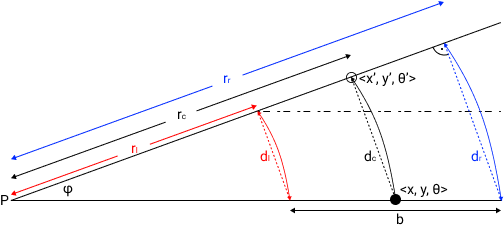
\includegraphics[width=0.8\linewidth]{img/odom}
	\caption{
		This diagram shows the geometry of how a slight turning motion can be calculated only using the distances $d_{l}$, $d_{r}$ and wheel offset $b$.
		The robot pose 
		$
			\begin{pmatrix}
				x &
				y &
				\theta 
			\end{pmatrix}^{T}
		$
		is associated with the center of the robot.
	}
	\label{fig:odom}
\end{figure}


\subsection{Inertial Measurement}
Another way of modelling motion usually utilized when a robot is not equipped with wheel encoder nor wheels is based on velocities influencing the vehicle. Typically the inputs of velocity based motion models are measured used Inertial Measurement Units (IMU), Gyroscopes and Accelerometers. 

These velocities $v$ and $\omega$ as the translational, linear and angular velocity are referred to as controls for the system. 
In contrast to odometry which can only be calculated after a movement has been performed these controls allow for prior motion planning. \footcite[Pages 92 - 99]{thrun2002probabilisticRobotics}

If these velocities stay fixed for the entire duration $\Delta t$ of the motion from 
$\begin{pmatrix} x & y & \theta \end{pmatrix}^{T}$
to
$\begin{pmatrix} x' & y' & \theta' \end{pmatrix}^{T}$
the robot moves in a circle with radius $r$ as seen in Fig. \ref{fig:inertial}. The center $P$ of this circle with coordinates 
$
\begin{pmatrix}
	x_{P} & y_{P}
\end{pmatrix}
^{T}
$
can be evaluated as follows:

\begin{equation}
	\begin{split}
		x_{P} = x - \frac{v}{\omega} \sin \theta \\
		y_{P} = y + \frac{v}{\omega} \cos \theta
	\end{split}
\end{equation}

This allows for the new position to be calculated: 

\begin{equation}
	\begin{pmatrix}
		x' \\
		y' \\
		\theta'
	\end{pmatrix}
	=
	\begin{pmatrix}
		x_{P} + \frac{v}{\omega} \sin(\theta + \omega \Delta t) \\
		y_{P} - \frac{v}{\omega} \cos(\theta + \omega \Delta t) \\
		\theta + \omega \Delta t
	\end{pmatrix}
\end{equation}

Despite incapable of calculating movements in advance, odometry ought to be preferred over velocity motion models as they pose higher accuracy in localization. \footcite[Page 107]{thrun2002probabilisticRobotics}

\begin{figure}
	\centering
	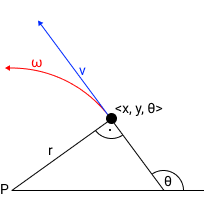
\includegraphics[width=0.5\linewidth]{img/inertial}
	\caption{
		In this diagram a slight turning motion of the robot is described by the translational velocity $v$ and angular velocity $\omega$. These velocities if consistent render the robot to move in a perfect circle with center $P$ and radius $r = | \frac{v}{\omega}|$. Even if the angular velocity remains 0 the motion is still described as a circle with an infinite radius.
	}
	\label{fig:inertial}
\end{figure}



\section{Depth Sensing}
Similar to motion models contributing to robot localization in Autumn, Depth Sensing is utilized to perceive and map the drones environment. 
The technologies in this section focus on mapping distance information to each point in the cameras field of view thus providing 3D-Imaging.

\subsection{Structured Light}
One approach uses active illumination to project a varying intensity pattern onto the perceived scene thus allowing for a camera to extract 3D-information from the distorted pattern as the surface of the scene is non-planar. \footcite{geng2011StructuredLight}

\subsection{Time-of-Flight}
Time-of-Flight (ToF) sensors perform active triangulation, meaning they are capable of retrieving depth information using only one camera, as seen in Fig. \ref{fig:activeTriangulation}. These sensors emit a modulated ray of light. The time it takes for the light to be reflected and detected by the camera is used to calculate the relative distance to a target. 
It may be necessary to differentiate mapping using depth perception sensors from LiDAR technologies which pose an alternative solution. 
Although LiDAR sensors fall under the category of ToF sensors they perceive the distance to an object using pulsed lasers thus outputting a point cloud rather than additional depth-information mapped to an image.\footcite{gokturk2004time} \footcite{velodyne2021LiDAR}
As 3D-LiDAR sensors applied in many commercial mapping solution are very expensive they disqualify for use in Autumn as it focuses on performing with approximate precision using relatively inexpensive camera based equipment. 

\subsection{Stereo Vision}
The last and most significant approach to Autumn performs passive triangulation using two cameras. Although this eliminates the need for any light to be emitted however the problem of correspondence is introduced, which deals with associating the different projections to the same point in the real world. There are multiple approaches to this problem which are generally divided into global and local matching methods with the latter being more computationally efficient while sacrificing quality.\footcite{do2019review}

In Autumn this approach was pursued using a Stereolabs ZED depth camera as it was superior to any competitors such as the Microsoft Kinect or Intel Realsense concerning availability and cost-effectiveness. 

\subsubsection{ZED 1 vs ZED 2}
%As mentioned in Chapter \ref{chapter:architecture} the Stereolabs ZED 1 was used in a first prototype and later replaced with a 





\filbreak